\documentclass{article}
\usepackage[utf8]{inputenc}
\usepackage{polski}
\usepackage{amsmath,amssymb,graphicx,subfig,pdfpages,enumitem,empheq,verbatim}

\author{Krystian Baran 145000}
\title{Sprawozdanie Lab 2 - Lab 6}

\begin{document}

\maketitle
\newpage

\tableofcontents
\newpage

{
\topskip0pt
\vspace*{\fill}
Do każdego zestawu zostało dodane cel ćwiczeń i krótki opis uzyskanej wiedzy. Do każdego zadania także został dodany krótki opis. Niektóre zadania mogą różnić się od wersji przesłanej na odpowiadające laboratoria.
\vspace*{\fill}
}

\newpage
\part{Laboratoria 2 - Rozkłady typu dyskretnego (Rozkład Dwumianowy)}

Celem tych laboratoriów było zapoznanie się z wybranymi rozkładami typu dyskretnego poprzez zestaw zadań i opracowanie jednego z dostępnych rozkładów
wyznaczając definicje, własności dostępne funkcje w różnych programach komputerowych i wymyślenie przykładu dla tego rozkładu.
Opracowany został rozkład dwumianowy z wymyślonym do niego przykładem. \\ \par
Za pomocą tych laboratoriów uzyskana została wiedza na temat różnych dostępnych funkcji, i osobiście, został wzbudzony interes do korzystania z języku programowania R ponieważ jest on rozszerzony w dużo funkcji statystycznych.

\section{Definicja}
\begin{flushleft}
Rozkład dwumianowy to rozkład prawdopodobieństwa zmiennej losowej x typu dyskretnego z parametrami $n$ i $p$. $n$ to liczba niezależnych od siebię prób przy których możliwe są tylko dwa wyniki odpowiednio z prawdopodobieństwem $p$ i $1-p$. Rozkład taki definiowany jest następującą funkcją:
$$f_{bin}(x|n,p) = \binom{n}{x}p^x(1-p)^{n-x}$$
gdzie $x = 0,1,\dots,n$. \\
Wartość oczekiwana wynosi $np$. Wariancja wynosi $np(1-p)$.
\end{flushleft}

\section{Funkcje}
\subsection{Excel}
W MS Excel dostępna jest funkcja aby obliczyć rozkład dwumianowy i dystrybuantę rozkładu dwumianowego dla danych parametrów i dla danego x. Funkcja ta jest następująca:
\begin{center}
BINOM.DIST(number\_s,trials,probability\_s,cumulative).
\end{center}
\begin{itemize}
\item\textbf{number\_s} - jest liczba $x$. 
\item\textbf{trials} - jest liczba prób, czyli $n$. 
\item\textbf{probability\_s} - jest prawdopodobieństwo sukcesu czyli p. 
\item\textbf{cumulative} - przyjmuje wartości 0 lub 1, i oznacza czy liczymy prawdopodobieństwo dla danego $x$ lub liczymy dystrybuantę dla danego $x$. 
\end{itemize}

\subsection{R}
W języku programowania R są dostępne funkcje obliczające rozkład dwumianowy dystrybuantę i kwartyle. 
\begin{enumerate}
\item dbinom(x, size, prob) - funkcja rozkładu dwumianowego
\item pbinom(x, size, prob) - dystrybuanta rozkładu dwumianowego
\end{enumerate}
\begin{itemize}
\item\textbf{x} - jest wartosć $x$ dla której liczymy rozkład 
\item\textbf{size} - jest liczba prób, czyli $n$ 
\item\textbf{prob} - jest prawdopodobieństwo sukcesu, czyli $p$ 
\end{itemize}

\subsection{Octave}
Dla GNU Octave potrzebne jest zainstalować pakiet "statistics" wraz z pakietem "io" który jest wymagany dla pakietu "statistics". W tym pakiecie dostępne są funkcje, jak poprzednio, obliczające wartości rozkładu dwumianowego i dystrybuantę.
\begin{enumerate}
\item binopdf(x, n, p)
\item binocdf(x, n, p)
\end{enumerate}
Parametry funkcji są samowyjasniające.

\subsection{Inne języki programowania}
Dla dowolnego języka programowania można napisać program wyliczający wartość funkcji rozkładu dwumianowego korzystając z następującego pseudokodu:
{\fontfamily{pcr}\selectfont \begin{tabbing}
def \= binomial\_coefficient(n, k) \+ \\
    if \= k $<$ 0 or k $>$ n: \\
    \>    return \= 0 \\
    if k $>$ n - k: \\
     \> \=   k = n - k \\
    if k == 0 or n <= 1: \\
        \> \=return 1 \\
    return binomial\_coefficient(n - 1, k) + binomial\_coefficient(n - 1, k - 1)  \- \\
\\
def \= binomial\_distribution(x, n, p) \+ \\
return \= binomial\_distribution(n, x) * p\textasciicircum k * (1 - p)\textasciicircum (n - k)
\end{tabbing}
}
Funkcja "binomial\_coefficient" jest optymalną wersją przy której korzysta się z własności że $\binom{n}{k} = \binom{n}{n-k}$ i unika korzystania z dużych wartości dla małych liczb.

\section{Przykład}
Firma \textbf{Firmex} produkuje długopisy w maszynie przemysłowej. Prawdopodobieństwo, że maszyna wyprodukuje uszkodzony długopis wynosi 0.03. Jeżeli maszyna produkuje dziennie 1000 długopisów, jakie będzie prawdopodobieństwo, że maszyna wyprodukuje w jedną dobę co najwyżej 60 uszkodzonych długopisów? \par
Prawdopodobieństwo wyprodukowania uszkodzonego długopisu można przybliżyć rozkładem dwumianowym z parametrami $p = 0.03$ i $n = 1000$, ponieważ każdy długopis ma to samo prawdopodobieństwo bycia źle wyprodukowanym, nie zależnie od innych długopisów. \\
Zatem potrzebujemy obliczyć prawdopodobieństwo, że tych długopisów będzie co najwyżej 60, czyli liczba sukcesów będzie mniejsza lub równa 60:
$$P(X\leq60)=\sum_{k=0}^{60}\binom{1000}{k}p^k(1-p)^{1000-k}\sim0.9999997$$
Zatem pewne jest, że maszyna wyprodukuję co najwyżej 60 uszkodzonych długopisów.

\section{Lab 2 - Zadanie 2}
W tym zadaniu zapoznaliśmy się z rozkładem Poissona i wyznaczanie parametru $\lambda$ rozkładu z danymi warunkami. \\ \par

Ile średnio powinno przypadać rodzynków na bułeczkę, aby prawd., że w bułeczce znajdzie się choćby jeden rodzynek, było nie mniejsze niż 0,99? \\ \par

Niech $X$ będzie rozkładem Poissona opisujące liczbę rodzynek na bułeczkę. Prawdopodobieństwo że w bułeczce będzie więcej niż jedna rodzynka wyznacza się w następujący sposób:
\[ P(X >= 1) = 0.99 \]

Gęstość prawdopodobieństwa rozkładu Poissona definiowana jest w następujący sposób:
\[ \begin{array}{cc} P(X=k) = \frac{\lambda^ke^{-\lambda}}{k!} &, k =0,1,2,\dots,\infty \end{array} \]

Korzystając z własności prawdopodobieństwa otrzymujemy następujące równanie:
\[  P(X >= 1) = 1 - P(X<1) = 1 - P(X=0) = 0.99 \]
Zatem szukamy taki parametr $\lambda$ rozkładu Poissona dla którego spełnione jest to równanie.
\begin{align*}
P(X=0) & = \frac{\lambda^0e^{-\lambda}}{0!} = e^{-\lambda} = 0.01 \\
-\lambda & = \ln(0.01) \\
\lambda & = -\ln(0.01) \approx 4.605170186
\end{align*}
Zatem aby na prawdopodobieństwo że na bułeczkę przypadała no najmniej jedna rodzynka parametr $\lambda$ musi być większy od 4.605170.

\section{Lab 2 - Zadanie 3}
W tym zadaniu także wykorzystaliśmy rozkład Poissona, natomiast został użyty do obliczenia zadania MS Excel, w którym jest dostępny rozkład Poissona. \\ \par

Lekarz pełniący dyżur w pewnym szpitalu wzywany jest do pacjentów średnio 3 razy w ciągu nocy. Można przyjąć, że liczba wezwań podlega rozkładowi Poissona. Jakie jest prawd., że noc upłynie lekarzowi spokojnie? \\ \par

Niech $X$ będzie zmienna losowa opisująca ilość razy który w nocy jest lekarz wzywany na dyżur. Z treści zadania średnia ilość wzywań na noc jest 3, zatem, wiedząc że wartość oczekiwana rozkładu Poissona wynosi $\lambda$ przyjmujemy że jest ona 3. Można zatem wyliczyć szukane prawdopodobieństwo:
\[ P(X=0) \overset{EXCEL}{=} POISSON.DIST(0,3,0) \approx 0.049787068 \]
Zatem prawdopodobieństwo że lekarz spełni noc spokojne wynosi 4.98\%.

% Laboratoria 3
\newpage
\part{Laboratoria 3 - Rozkłady typu ciągłego (Rozkład Weibulla)}

Celem tych laboratoriów było zapoznanie się z dostępnymi funkcjami obliczające gęstość i dystrybuantę różnych rozkładów typu ciągłego poprzez rozwiązywanie różnych zadań i przeprowadzenie analizy jednego z tych rozkładów w różnych programach komputerowych. Wybrany przeanalizowany rozkład to rozkład Weibulla. \\ \par
Ukrytym celem laboratoriów był także sprawdzenie poprawności niektórych zadań z książki z której zadania zostały podane, ponieważ książka została napisana dawno temu i mogły się pewne błędy pojawić. Natomiast okazało sie że nie było większych błędów i zadania zostały poprawnie wykorzystane do sprawdzenia i wzbogacenia wiedzy w dostępnych funkcjach rozkładów typu ciągłego.

\section{Definicja}

Rozkład Weibulla jest rozkładem zmiennej losowej typu ciągłego, które bierze imię od Szwedzkiego matematyka, który pierwszy opisał w detalu ten o to rozkład. \par
Funkcja gęstości jest następująca: \\
$$f(x|k,\lambda) = \frac{k}{\lambda} \Big( \frac{x}{\lambda} \Big) ^{k-1} e^{-(x/\lambda)^k} \boldsymbol{1}_{[0,\infty]}(x)$$
Gdzie $k>0, \lambda>0$. \\

\subsection{Wartość oczekiwana}
$$E(X) = \int_{-\infty}^{\infty} x\frac{k}{\lambda} \Big( \frac{x}{\lambda} \Big) ^{k-1} e^{-(x/\lambda)^k} \boldsymbol{1}_{[0,\infty]}(x)dx = \int_{0}^{\infty} x\frac{k}{\lambda} \Big( \frac{x}{\lambda} \Big) ^{k-1} e^{-(x/\lambda)^k}dx=$$
$$\Big( \frac{x}{\lambda} \Big) ^k = u$$
$$dx = \frac{\lambda^{k}}{k\cdot x^{k-1}}du$$
$$\frac{k}{\lambda} \int_{0}^{\infty} \lambda u^{1/k} \frac{x^{k-1}} {\lambda^{k-1}} e^{-u} \frac{\lambda^{k}}{k\cdot x^{k-1}}du=$$
$$\lambda \int_{0}^{\infty}u^{(1+1/k)-1}e^{-u}=$$
$$\lambda \Gamma (1+\frac{1}{k})$$.

\subsection{Wariancja}
$$E(X^2) = \int_{-\infty}^{\infty} x^2 \frac{k}{\lambda} \Big( \frac{x}{\lambda} \Big)^{k-1} e^{-(x/\lambda)^k}  \boldsymbol{1}_{[0,\infty]}(x)dx = \int_{0}^{\infty} x^2 \frac{k}{\lambda} \Big( \frac{x}{\lambda} \Big)^{k-1} e^{-(x/\lambda)^k}$$
$$\Big( \frac{x}{\lambda} \Big) ^k = u$$
$$dx = \frac{\lambda^{k}}{k\cdot x^{k-1}}du$$
$$\frac{k}{\lambda} \int_{0}^{\infty} \lambda^2 u^{2/k} \frac{x^{k-1}} {\lambda^{k-1}} e^{-u} \frac{\lambda^{k}}{k\cdot x^{k-1}}du=$$
$$\lambda^2 \int_{0}^{\infty}u^{(1+2/k)-1}e^{-u}=$$
$$\lambda^2 \Gamma (1+\frac{2}{k})$$
\\
$$D^2(X) = E(X^2) - E(X)^2 = \lambda^2 \Gamma (1+\frac{2}{k}) - (\lambda \Gamma (1+\frac{1}{k}))^2 = \lambda^2 \Gamma (1+\frac{2}{k}) - \lambda^2 \Gamma (1+\frac{1}{k})^2=$$
$$\lambda^2 ( \Gamma (1+\frac{2}{k}) -  \Gamma^2 (1+\frac{1}{k}))$$

\section{Excel}
W programie MS Excel jest dostępna funkcja, która oblicza wartość funkcji gęstości i dystrybuanty rozkładu Weibulla. Jest to funkcja WEIBULL(x,alpha,beta,cumulative).
\begin{itemize}
\item \textbf{x} - to wartość zmiennej losowej.
\item \textbf{alpha} - to nasz parametr $k$ rozkładu.
\item \textbf{beta} - to nasz parametr $\lambda$ rozkładu.
\item \textbf{cumulative} - przyjmuje wartości 0 dla funkcji gęstości lub 1 dla dystrybuanty.
\end{itemize}

\newpage
\section{R}
W R dostępne są funkcje gęstości i dystrybuanty rozkładu Weibulla i są to odpowiednio:
\begin{itemize} 
\item dweibull(x, shape, scale = 1, log = FALSE)
\item pweibull(q, shape, scale = 1, lower.tail = TRUE, log.p = FALSE)
\end{itemize}
Gdzie:
\begin{itemize}
\item \textbf{x,q} - to wartość zmiennej losowej.
\item \textbf{shape} - to nasz parametr $k$ rozkładu.
\item \textbf{scale} - to nasz parametr $\lambda$ rozkładu.
\end{itemize}

\section{Octave}
W pakiecie "Statistics" dostępne są, jak powyżej, funkcję obliczające wartość funkcji gęstości i dystrybuanty rozkładu Weibulla. Są to funkcje, odpowiednio:
\begin{itemize} 
\item wblpdf(x, scale, shape)
\item wblcdf(x, scale, shape)
\end{itemize}
gdzie:
\begin{itemize}
\item \textbf{x} - to wartość zmiennej losowej.
\item \textbf{scale} - to nasz parametr $\lambda$ rozkładu.
\item \textbf{shape} - to nasz parametr $k$ rozkładu.
\end{itemize}

\section{Przykład}
Prędkość wiatru w danej miejscowości ma rozkład Weibulla z parametrami $k = 2, \lambda = 8$ w $[\frac{m}{s}]$. Obliczyć najbardziej prawdopodobną prędkość wiatru i prawdopodobieństwo że prędkość wiatru będzie mniejsza niż $4 [\frac{m}{s}]$. \par
$$E(X) = \lambda \Gamma(1+\frac{1}{k}) = 8\cdot \Gamma(1+\frac{1}{k}) =8\cdot \Gamma(\frac{3}{2}) \approx 8\cdot 0.8862269 \approx 7.089815 [\frac{m}{s}]$$
$$P(X<4) = F(4) \approx 0.2211992$$
%\begin{figure}[h]
\begin{center}
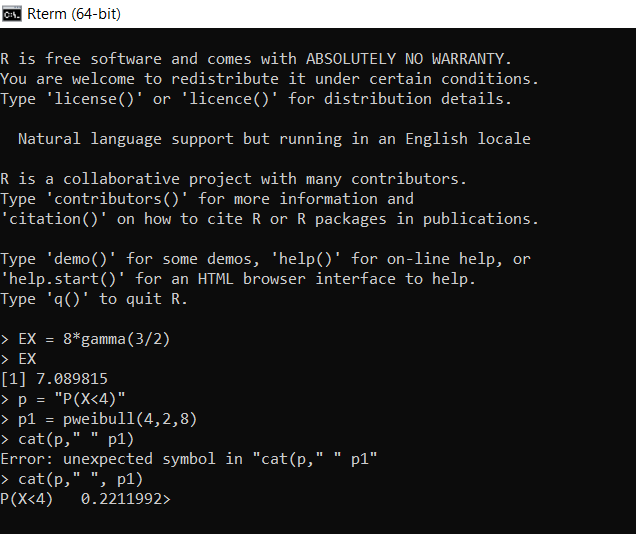
\includegraphics[width=1\textwidth, angle=0]{image2Weibull.png}
\end{center}
%\centering
%\end{figure}
Zatem najbardziej prawdopodobną prędkość wiatru w tej miejscowości wynosi $7 \frac{m}{s}$ a prawdopodobieństwo że prędkość wiatru będzie mniejsza niż 4 wynosi około $0.22$.

\section{Lab 3 - Zadanie K 2.27}
W tym zadaniu został wykorzystany skrypt R-owski zatem zagłębiona została wiedza w tworzeniu wykresów i tworzeniu funkcji w R, ponieważ podany w zadaniu rozkład nie był dostępnym, lub nie został znaleziony. \\ \par

Przedstawić krzywe gęstości rozkładu Erlanga oraz obliczyć prawdopodobieństwo
$P(1 < X < 2)$ dla: 
\begin{itemize}
\item $X \sim ERL(2, 1)$,
\item $X \sim ERL(2, 5)$.
\end{itemize}

Rozkład Erlanga jest rozkładem dla zmiennej losowe typu ciągłego z następującą funkcją gęstości:
\[\begin{array}{cc} f(x;k,\lambda) = \frac{\lambda^kx^{k-1}e^{-\lambda}}{(k-1)!}, & x,\lambda > 0 \end{array} \]

Zadanie to zostało rozwiązane za pomocą skryptu R-owskiego przedstawionego poniżej gdzie zdefiniowana została funkcja obliczająca gęstość rozkładu Erlanga. Natomiast jej dystrybuanta nie została wyznaczona ale prawdopodobieństwa zostały wyliczone za pomocą funkcji całkującej; wybrana metoda całkowania to metoda całkowania Kronroda o której nie będziemy mówić.

{{\fontfamily{pcr}\selectfont
\begin{tabbing}
library(pracma) \\
X = "ERL(2,1)" \\
X1 = "ELR(2,5)" \\
erl \= = function(x,a,b) \{ \+ \\
	erl = b\textasciicircum a*x \textasciicircum(a-1)/gamma(a)*exp(-b*x) \- \\
\} \\
x = seq(0,10,by = 0.01) \\
y = erl(x,2,1) \\
y1 = erl(x,2,5) \\
Y $<$- function(x) erl(x,2,1) \\ 
Y1 $<$- function(x) erl(x,2,5) \\
png(file = "zad2\_27\_f1.png") \\
plot(x,y1,type = "l", xlab = "x", ylab = "y") \\
lines(x,y, col ="green") \\
dev.off() \\
p = integral(Y,1,2, method = "Kron") \\
p1 = integral(Y1,1,2, method = "Kron") \\
cat(X," P(1$<$X$<$2) = ",p,"\textbackslash n") \\
cat(X1," P(1$<$X$<$2) = ",p1,"\textbackslash n") \\
\end{tabbing}
}
Program ten zwraca szukane wartości i wykresy:
\begin{itemize}
\item ERL(2,1)  P(1$<$X$<$2) =  0.329753 
\item ELR(2,5)  P(1$<$X$<$2) =  0.03992828
\end{itemize}

Wykres generowany przez program jest następujący, czarna funkcja to ERL(2,5) natomiast zielona to ERL(2,1).
\newpage
{
\topskip0pt
\vspace*{\fill}
\begin{figure}[h!]
\begin{center}
\includegraphics[height = 0.5\textheight]{"zad2_27_f1.png"}
\end{center}
\end{figure}
\vspace*{\fill}
}

% Laboratoria 4
\newpage
\part{Laboratoria 4 - Rozkład normalny}

Celem tych laboratoriów było zapoznanie się z metodami komputerowymi i tablicowymi obliczania rozkładu normalnego poprzez zadania; zapoznanie się z przykładowym zadaniem który mógł by się pojawić na kolokwium zaliczeniowe. \\
Studium przypadku było zadanie obszerne gdzie trzeba było także skorzystać z podanego rozkładu i stworzyć nową zmienną losową innego rozkładu, tym razem typu dyskretnego; zatem zagłębiona została wiedza rozkładu normalnego a także już wcześniej wykorzystanych rozkładów a także metod komputerowego rozwiązywania zadań.

\section{Przykład projektu zaliczeniowego cz 1}
Długość $X$ (w [mm]) detalu produkowanego na pewnym automacie jest zmienną losową o gęstości prawdopodobieństwa
$$f_{X}(x) = \frac{1}{\sigma\sqrt{2\pi}}\exp\Big(\frac{-x^2+40x-400}{0.08}\Big), x\in\mathbb{R}$$

\begin{enumerate}
\item Rozpoznać rozkład długości detalu i jego parametry, wyznaczyć drugi moment zwykły długości detalu, sporządzić krzywą gęstości i dystrybuantę.
\item Obliczyć prawd. zdarzeń: $|X-19.98|\geq 0.02$, $|X-\mathbb{E}X|<\mathbb{D}X$.
\item Dla jakiej wartości stałej $b$ zachodzi równość $P(x_{0.05}<X<b)=0.90$?
\item Wyznaczyć kwartyle długości detalu oraz obliczyć wartości gęstości dla nich.
\item Wyznaczyć przedział, w którym mieści się 95\% produkowanych detali po złomowaniu 5\% detali o największej odchyłce długości od wymiaru przeciętnego.
\item Co wynika z faktu, że łączna długość 180 wyprodukowanych detali będzie mniejsza od 358[cm]?
\item Detal spełnia normę długości, jeśli jego długość mieści się w dopuszczalnym przedziale (19,6; 20,4) [mm]. W celu sprawdzenia dokładności produkcji zmierzona zostanie długość 180 losowo wybranych detali.
\begin{enumerate}
\item Wprowadzić zmienną losową opisującą wynik sprawdzania normy długości badanej partii detali. Podać jej rozkład i sporządzić wykresy PMF i CDF.
\item Obliczyć prawd. zdarzenia, że w badanej partii detali, co najmniej 175 z nich spełni normę długości.
\item Wyznaczyć wartość oczekiwaną, odchylenie standardowe oraz modę liczby detali, które spełnią normę długości i prawdopodobieństwo dla mody.
\end{enumerate}
\end{enumerate}

\subsection{1)}
Korzystając z przekształceń funkcję gęstości sprowadza się to funkcji gęstości rozkładu normalnego z parametrami $\mu$ i $\sigma$.
$$\frac{1}{\sigma\sqrt{2\pi}}\exp\Big(\frac{-x^2+40x-400}{0.08}\Big) = \frac{1}{\sigma\sqrt{2\pi}}\exp\Big(-\frac{(x-20)^2}{2\cdot(0.2)^2}\Big)$$
$$N(\mu,\sigma) = \frac{1}{\sigma\sqrt{2\pi}}\exp\Big(-\frac{(x-\mu)^2}{2\cdot\sigma^2}\Big)$$
Zatem $\mu = 20$ i $\sigma = 0.2$.

\subsection{2)}
Dla $|X-19.98|\geq 0.02$:
\begin{align*}
P(|X-19.98|\geq0.02) & = 1 - P(|X-10.98|<0.02) \\
& = 1 - P(-0.02<X-19.98<0.02) \\
& = 1 - P(19.96<X<20) \\
& = 1 - F_{N(20,0.2)}(20) + F_{N(20,0.2)}(19.96) \\
& \overset{R}{=} 1 - pnorm(20,20,0.2) + pnorm(19.96,20,0.2) \\
& \approx 1 - 0.5 + 0.4207403 \approx 0.9207403
\end{align*}
Gdzie $pnorm(x,\mu,\sigma)$ to funkcja z R obliczająca wartość dystrybuanty rozkładu normalnego dla danego $x$ i z danymi parametrami $\mu$ i $\sigma$.
\\
\par
Dla $|X-\mathbb{E}X|<\mathbb{D}X$ wiemy że $\mu = \mathbb{E}X$ i że $\sigma = \mathbb{D}X$. Zatem:
\begin{align*}
P(|X-\mathbb{E}X|<\mathbb{D}X) & = P(|X-20|<0.2) = P(-0.2<X-20<0.2) \\
& = P(19.8<X<20.2) \\
& = F_{N(20,0.2)}(20.2) - F_{N(20,0.2)}(19.8) \\
& \overset{R}{=} pnorm(20.2,20,0.2) - pnorm(19.8,20,0.2) \\
& \approx 0.8413447 - 0.1586553 \approx 0.6826894
\end{align*}
Gdzie $pnorm()$ to ta sama funkcja co wcześniej. \\
Zatem $P(|X-19.98|\geq0.02) = 0.92$ a $P(|X-\mathbb{E}X|<\mathbb{D}X) = 0.68$.

\subsection{3)}
Dowolny kwantyl rozkładu normalnego wyznacza się za pomocy standardowego rozkładu normalnego, to znaczy:
$$x_{p} = \mu + \sigma\Phi^{-1}(p)$$
Zatem, podstawiając $Z = \frac{X-20}{0.2} \sim N(0,1)$
\begin{align*}
P(x_{0.05}<X<b) & = P\Big(\frac{x_{0.05}-20}{0.2}<\frac{X-20}{0.2}<\frac{b-20}{0.2}\Big) \\
& =  \Phi\Big(\frac{b-20}{0.2}\Big) - \Phi\Big(\frac{x_{0.05}-20}{0.2}\Big) \\
& =  \Phi\Big(\frac{b-20}{0.2}\Big) - \Phi\Big(\frac{20+0.2\cdot\Phi^{-1}(0.05)-20}{0.2}\Big) \\
& =  \Phi\Big(\frac{b-20}{0.2}\Big) - 0.05 = 0.9
\end{align*}
$$ \Phi\Big(\frac{b-20}{0.2}\Big) = 0.95$$
$$\frac{b-20}{0.2} = \Phi^{-1}(0.95)$$
$$b = 20 + 0.2\cdot\Phi^{-1}(0.95) = x_{0.95}$$
Zatem $b \overset{R}{=} qnorm(0.95, 20, 0.2) \approx 20.32897$.

\subsection{4)}
Kwartyle wyznaczamy za pomocą funkcji z R $qnorm(p,\mu,\sigma)$ która oblicza wartość kwartylu $p$ dla podanych $\mu$ i $\sigma$.
\begin{align*}
x_{0.25} & = qnorm(0.25,20,0.2) = 19.8651 \\
x_{0.5} & = qnorm(0.5,20,0.2) = 20 \\
x_{0.75} & = qnorm(0.75,20,0.2) = 20.1349
\end{align*}
\\
Wartości gęstości w tych punktach są następujące:
$$f_{N(20,0.2)}(19.8651) = dnorm(19.8651,20,0.2) = 1.588872$$
$$f_{N(20,0.2)}(20) = dnorm(20,20,0.2) = 1.994711$$
$$f_{N(20,0.2)}(20.1349) = dnorm(20.1349,20,0.2) = 1.588872$$
Gdzie $dnorm(x,\mu,\sigma)$ to funkcja Z R obliczająca wartość funkcji gęstości w danym $x$ i danymi parametrami $\mu$ i $\sigma$.

\subsection{5)}
Szukany przedział gdzie mieści się 95\% detali po złomowaniu najbardziej odchylonych od wartości przeciętnej 5\% będzie przedziałem środkowym. Ponieważ nie możemy złomować 5\% tylko na końcu lub na początku całej zbiorowości, złomujemy równomiernie 2.5\% na początku i na końcu. Wtedy, aby znaleźć szukany przedział wystarczy obliczyć kwantyle rzędu 0.025 z prawej i z lewej strony przedziału. Obliczymy to funkcją R-owską co pozwala na obliczenie z prawej i z lewej dany kwantyl. Oznaczmy przedział jako $(a,b)$.
\begin{align*}
a & \overset{R}{=} qnorm(0.025, 20, 0.2) \approx 19.60801 \\
b & \overset{R}{=} qnorm(0.025, 20, 0.2, lowe.tail = FALSE) \approx 20.39199
\end{align*}
Zatem szukany przedział gdzie mieści się 95\% detali jest $(19.61, 20.39)$.

\subsection{6)}
Według centralnego twierdzenia granicznego, rozkład sumy $n$ rozkładów normalnych z parametrami $\mu,\sigma$ jest $\sim N(n\cdot \mu, \sigma\sqrt{n})$.
Zatem dla 180 detali rozkład sumy będzie następujący:
\[ Y = \sum_{i=1}^{180} X_i \sim N(180\cdot20, 0.2\sqrt{180}) = N(3600, \sqrt{7.2}) \]
Obliczymy prawdopodobieństwo że suma detali będzie mniejsza od 3580 [mm].
\[ P(Y<3580) \overset{R}{=} pnorm(3580, 3600, sqrt(7.2)) \approx 4.542735e-14 \]
Prawdopodobieństwo jest bardzo małe zatem dana wartość oczekiwana i wariancja jest poprawnie podana; gdyby to prawdopodobieństwo było duże oznaczało by to że podane parametry rozkładu są nie poprawne, zatem albo wybraliśmy za dużą wartość oczekiwaną lub za małe odchylenie standardowe.

\subsection{7)}
Załóżmy ze każdy detal produkowany jest niezależnie; wtedy prawdopodobieństwo wyprodukowania $k$ detali 
które mieszczą się w przedziale będzie miało rozkład dwumianowy z parametrami $n = 180$ i $p = P(19.6<X<20.4)$.
\[
	P(Y=k) = \binom{180}{k}p^k\cdot(1-p)^{180-k}, k=0,1,2\dots.
\]
Jako pierwsze trzeba obliczyć p. 
\begin{align*}
p & = P(19.6<X<20.4) \\
& = F_{N(20,0.2)}(20.4) - F_{N(20,0.2)}(19.6)  \\
& \overset{R}{=} pnorm(20.4,20,0.2) - pnorm(19.6,20,0.2)  \\
& \approx 0.9772499 - 0.02275013 \approx 0.9544997
\end{align*}
Zatem $p = 0.95$. 
Wykres gęstości i dystrybuanty zostały sporządzone w R i wyglądają następująco:
\begin{figure}[h!]
\begin{center}
\includegraphics[height=0.35\textheight, angle=0]{"lab4zad1_d.png"}
\caption{Gęstość}
\end{center}
\end{figure}

\begin{figure}[h!]
\begin{center}
\includegraphics[height=0.35\textheight, angle=0]{"lab4zad1_f.png"}
\caption{Dystrybuanta}
\end{center}
\end{figure}

\newpage
Prawdopodobieństwo, że co najmniej 175 detali spełni normę jest następujące:
\begin{align*}
	P(Y\geq175) & = 1 - P(Y<175) \\
	& \overset{R}{=} 1 - pbinom(175,180,0.95) \\
	& \approx 1 - 0.9492507 \approx 0.05074934
\end{align*} \\
Zatem prawdopodobieństwo wykonania, co najmniej 175 detali według normy wynosi 0.05.
\par
Wartość oczekiwana zmiennej losowej Y wynosi:
$$\mathbb{E}Y = n\cdot p = 180\cdot0.95 = 171$$
\par
Variancja zmiennej losowej Y wynosi:
$$\mathbb{D}^2(Y) = n\cdot p\cdot(1-p) = 180\cdot 0.95\cdot0.05 = 85.5$$
\par
Odchylenie standardowe zmiennej losowej Y wynosi:
$$\mathbb{D}Y = \sqrt{85.5} \approx 9.2466$$
\par
Aby obliczyć wartość modalną sprawdzimy warunek: $(n+1)p = 181\cdot 0.95 = 171.95$. 
Jest to liczba rzeczywista, zatem wartość modalna wynosi 171.
\par
Prawdopodobieństwo, że wyprodukujemy dokładne wartość modalna odcinków spełniających normę wynosi:
$$P(Y=171) = dbinom(171,180,0.85) = 0.1351751$$
Gdzie $dbinom(k,n,p)$ to funkcja z R obliczająca wartość gęstości dla danego $k$ i danych parametrów $n$ i $p$.

\section{Lab 4 - Zadanie 4}
W tym zadaniu została wykorzystana wiedza o normalizacji rozkładu normalnego w celu skorzystania z tabeli ponieważ parametry nie były podane. Została także wykorzystana wiedza wartości oczekiwanej rozkładu dyskretnego wraz z wiedzą tworzenia rozkładu gęstości. \\ \par

Opór $R$ pewnego typu oporników elektrycznych można opisać rozkładem normalnym $N(\mu,\sigma)$. Koszt produkcji jednego opornika wynosi $k$, jego cena rynkowa zaś równa jest $5k$, gdy $R\in(\mu - \sigma,\mu + \sigma)$ i $2k$, jeżeli $R\in(\mu-2\sigma,\mu-\sigma)$ lub $R\in(\mu+\sigma,\mu+2\sigma)$. Oporniki, które nie spełnią podanych kryteriów, nie mogą być sprzedawane. Oblicz dochód na jeden opornik.
\\
\par
Jako pierwsze trzeba obliczyć prawdopodobieństwa, że rezystancja $R$ będzie znajdować się w danych przedziałach. Oznaczymy je, jako $p1$, $p2$ i $p3$.
$$p1 = P(\mu - \sigma< X < \mu + \sigma) = P\Big(\frac{\mu - \sigma - \mu}{\sigma} < \frac{X-\mu}{\sigma} < \frac{\mu + \sigma - \mu}{\sigma}\Big)$$
Wtedy $\frac{X-\mu}{\sigma} \sim N(0,1)$, zatem:
$$P\Big(-1<\frac{X-\mu}{\sigma}<1\Big) = \Phi(1) - \Phi(-1) = 2\cdot\Phi(1) - 1 \approx 2\cdot0.8413 - 1 \approx 0.6826$$
\par
Ponieważ 
$$P(\mu-2\sigma<X<\mu+2\sigma) = p1 + P(\mu-2\sigma<X<\mu-\sigma \vee \mu+\sigma<X<\mu+2\sigma) = p1 + p2$$
to:
\begin{align*}
p2 & = P(\mu-2\sigma<X<\mu+2\sigma) - p1 \\
& = P\Big(\frac{\mu - 2\sigma - \mu}{\sigma}<\frac{X-\mu}{\sigma}<\frac{\mu+2\sigma-\mu}{\sigma}\Big) - p1 \\
& = \Phi(2) - \Phi(-2) - p1 = 2\cdot\Phi(2) - 1 - p1 \\
& \approx 2\cdot0.97725 - 1 - 0.6826 \approx 0.2719
\end{align*}
\par
Skoro $p1 + p2 + p3 = 1$ to można łatwo obliczyć $p3$:
$$p3 = 1 - p1 - p2 = 1 - 0.6826 - 0.2719 \approx 0.0455$$

\par
Można teraz sporządzić tabele rozkładu dyskretnego opisującego dochód dla jednego rezystora
\begin{center}
\begin{tabular}{|c|c|c|c|}
\hline
$x_i$ & 4k & k & -k \\
\hline
$P(X = x_i)$ & 0.6826 & 0.2719 & 0.0455\\
\hline
\end{tabular}
\end{center}
\par
Z definicji wartości oczekiwanej można obliczyć spodziewany dochód na rezystora.
$$\mathbb{E}X = \sum_{i=1}^{n}x_i\cdot P(X=x_i) = 4k\cdot0.6826 + k\cdot0.2719 - k\cdot0.0455 =$$
$$k\cdot(4\cdot0.6826 + 0.2719 - 0.0455) \approx k\cdot 2.9576$$
Zatem możemy się spodziewać dochód 3 razy większy niż cena produkcji rezystora.

% Laboratoria 5
\newpage
\part{Laboratoria 5 - Podstawy statystyki matematycznej}
Celem tych laboratoriów było zagłębienie wiedzy już znanych rozkładów a także zapoznanie się z centralnym twierdzeniem granicznym i przybliżeniem rozkładów rozkładem normalnym. Zagłębiona została także wiedza w wspomaganiu komputerowym do obliczenia danych zadań.

\section{Lab 5 - Zadanie 4}
Niech $X_1, \dots , X_n$ będzie próbą prostą z populacji, w której
cecha $X$ ma rozkład o gęstości
\[
f(x) = \frac{x}{8} \textbf{1}_{(0,4)}(x)
\]
\begin{enumerate}[label = \alph*)]
\item Wyznaczyć dystrybuantę i gęstość statystyk\\ $Y = max\{X_1,\dots, X_n\}$, $Z = min\{ X_1,\dots ,X_n \}$.
\item Obliczyć prawd. zdarzeń $Y<3$, $X>1$.
\item Obliczyć wartości oczekiwane i wariancje $Y$ i $Z$.
\end{enumerate}

\subsection{a)}
Załóżmy że $X_1,\dots,X_n$ są niezależne. Jeżeli maksymalna z wybranych liczb musi być mniejsza od pewnej liczby, to każda inna od maksymalnej też musi być od niej mniejsza. Wtedy dystrybuantę $F_Y$ można wyznaczyć następująco:
\[
F_Y(t) = P(Y\leq t) = \prod_{i=1}^{n} P(X_i \leq t) = P(X_i \leq t)^n
\]
Dla $t \in (0,4)$:
\begin{align*}
P(X_i \leq t) & = \int_{-\infty}^{t} \frac{x}{8} \textbf{1}_{(0,4)}(x) dx \\
& = \int_{0}^{t} \frac{x}{8} dx = \frac{x^2}{16} \Big\vert_{0}^{t} \\
& = \frac{t^2}{16}
\end{align*}

Zatem dystrybuanta przyjmuje następujący rozkład:
\[
F_Y(t) = \left\{
\begin{array}{ll}
0 &, t \leq 0 \\
\Big( \frac{t^2}{16} \Big)^n &, 0<t<4 \\
1 &, t \geq 4
\end{array}
\right.
\]

Korzystając z wiedzy, że funkcja gęstości to pochodna dystrybuanty, można ją wyznaczyć:
\[
f_Y(x) = \frac{F_Y(x)}{dx}
\]

\[
f_Y(x) = \left\{
\begin{array}{ll}
0 &, x \leq 0 \\
n \Big( \frac{x^2}{16} \Big)^{n-1} \frac{x}{8} &, 0<x<4 \\
0 &, x \geq 4
\end{array}
\right.
\]

Dla $Z$ natomiast, jeżeli minimalna liczba musi być większa od danej liczby, to każda inna od minimalnej też musi być od niej większa. Zatem można wyznaczyć dystrybuantę:

\[
F_Z(t) = P(Z \leq t) = 1 - P(Z > t) = 1 - \prod_{i=1}^{n} P(X_i > t) = 1 - ( 1 - P(X_i \leq t) )^n
\]

Więc, korzystając z poprzedniej wyliczonej całki, dystrybuanta przyjmuje następujący rozkład:
\[
F_Z(t) = \left\{
\begin{array}{ll}
0 &, t \leq 0 \\
1 - \Big(1 - \frac{t^2}{16} \Big)^n &, 0<t<4 \\
1 &, t \geq 4
\end{array}
\right.
\]

Funkcja gęstości będzie miała natomiast taki rozkład:

\[
f_Z(x) = \left\{
\begin{array}{ll}
0 &, x \leq 0 \\
n \Big(1 - \frac{x^2}{16} \Big)^{n-1} \frac{x}{8} &, 0<x<4 \\
0 &, x \geq 4
\end{array}
\right.
\]

\subsection{b)}
Ponieważ wyliczona została już dystrybuanta dla $Y$ i dla $Z$, to można łatwo obliczyć szukane prawdopodobieństwa:

\[
P(Y<3) = F_Y(3) = \Big( \frac{9}{16} \Big)^n
\]

Jeżeli $n \rightarrow \infty$ to $P(Y<3) \rightarrow 0$ oznacza to, że wartość maksymalna całkowita jest większa od 3\\

\begin{align*}
P(Z>1) & = 1 - P(Z<1) = 1 - F_Z(1) = 1 - \Big( 1 - \Big( 1 - \frac{1}{16} \Big)^n \Big)  \\
& = \Big( \frac{15}{16} \Big)^n
\end{align*}

Jeżeli $n \rightarrow \infty$ to $P(Z>1) \rightarrow 0$ oznacza to, że wartość minimalna całkowita jest mniejsza od 1.

\subsection{c)}
Zaczniemy od obliczenia wartości oczekiwanej $Y$.

\begin{align*}
\mathbb{E}Y & = \int_{\mathbb{R}}^{} n\cdot x \Big( \frac{x^2}{16} \Big)^{n-1} \frac{x}{8} \textbf{1}_{(0,4)}(x) dx \\
& = \int_{0}^{4} n\cdot x \Big( \frac{x^2}{16} \Big)^{n-1} \frac{x}{8} dx \\
& = \frac{n}{16^{n-1}8} \int_{0}^{4} x^{2n} dx \\
& =  \frac{n}{16^{n-1}8} \Big[ \frac{x^{2n+1}}{2n+1} \Big\vert_0^4 \\
& = \frac{n \cdot 4^{2n+1}}{4^{2n-2} \cdot 8(2n+1)} = \frac{8n}{2n+1}
\end{align*}

Jeżeli $n \rightarrow \infty$, to $ \mathbb{E}Y \rightarrow 4$, zatem wartość maksymalna dąży do granicy przedziału.\\
Następnie obliczymy wariancję $Y$.

\begin{align*}
\mathbb{E}(Y^2) & = \int_{\mathbb{R}}^{} n\cdot x^2 \Big( \frac{x^2}{16} \Big)^{n-1} \frac{x}{8} \textbf{1}_{(0,4)}(x) dx \\
& = \int_{0}^{4} n\cdot x^2 \Big( \frac{x^2}{16} \Big)^{n-1} \frac{x}{8} dx \\
&\begin{array}{c|c|c}
\hline
& D & I \\
+ & x^2 & n\cdot \Big( \frac{x^2}{16} \Big)^{n-1} \frac{x}{8} \\
- & 2x & \Big( \frac{x^2}{16} \Big)^n \\
\hline
\end{array} \\
& = x^2 \Big( \frac{x^2}{16} \Big)^n - \int_{0}^{4} 2x \Big( \frac{x^2}{16} \Big)^n dx \\
& = \Big[ x^2 \Big( \frac{x^2}{16} \Big)^n - \frac{16}{n+1} \Big( \frac{x^2}{16} \Big)^{n+1} \Big\vert_0^4 \\
& = 16 \Big( \frac{16}{16} \Big)^n - \frac{16}{n+1} \Big( \frac{16}{16} \Big)^{n+1} \\
& = \frac{16(n+1) - 16}{n+1} = \frac{16}{n+1}
\end{align*}

\[
\mathbb{D}^2(Y) = \mathbb{E}(Y^2) - \mathbb{E}Y^2 = \frac{16}{n+1} - \frac{64n^2}{(2n+1)^2}
\]

%oczekiwana z
Obliczymy teraz wartość oczekiwaną $Z$.
\begin{align*}
\mathbb{E}Z & = \int_{\mathbb{R}}^{} n\cdot x \Big(1 - \frac{x^2}{16} \Big)^{n-1} \frac{x}{8} \textbf{1}_{(0,4)}(x) dx \\
& = \int_{0}^{4} n\cdot x \Big(1 - \frac{x^2}{16} \Big)^{n-1} \frac{x}{8} dx 
\end{align*}

Jest to trudna do obliczenia całka, zatem, na podstawie wartości oczekiwanej jak poprzednio, wnioskujemy że wartość oczekiwana $\mathbb{E}Z$ będzie dążyć do 0 dla n dążącego do nieskończoności. \\
Ponieważ nie obliczyliśmy wartość oczekiwanej nie możemy obliczyć wariancję.

\section{Lab 5 - Zadanie 3}
W tym zadaniu wzbogacona została wiedza centralnego twierdzenia granicznego i wzbogacona została wiedza na temat rozkładu wartości maksymalnej ze zbioru. Także została wzbogacona wiedza na temat języka programowania R. \\ \par

Losujemy 100 liczb według rozkładu jednostajnego na
przedziale (0, 1).
\begin{enumerate}[label = \alph*)]
\item Ustalić rozkład sumy tych liczb.
\item Obliczyć prawd. zdarzenia, że suma wylosowanych
liczb nie będzie należała do przedziału (45, 55).
\item Wyznaczyć dystrybuantę największej z wylosowanych
liczb i oblicz prawd., że liczba ta będzie mniejsza od 0,95.
\item Jaki wniosek należy wyciągnąć, jeśli że suma wylosowanych liczb będzie mniejsza niż 40?
\end{enumerate}

\subsection{a)}
Niech $X_i$ będzie wylosowana i-ta liczba. $X_i \sim U(0,1)$ jest rozkładem jednostajnym na przedziale $(0,1)$ z następującą funkcją gęstości:
\[
f_{X_i}(x) = \left\{
\begin{array}{ll}
0 &, x \leq 0 \vee x \geq 1 \\
1 &, 0 < x < 1
\end{array}
\right. 
\]

Wtedy dystrybuanta przyjmuję następujący wzór:
\[
F_{X_i}(t) = \left\{
\begin{array}{ll}
0 &, t \leq 0 \\
t &, 0 < t < 1 \\
1 &, t \geq 1
\end{array}
\right. 
\]

Korzystając z centralnego twierdzenia granicznego dla sumy, przyjmując, że 100 jest wystarczającą dużą liczbą, rozkład sumy przyjmuje rozkład normalny z następującymi parametrami.
\[
X = \sum_{i=1}^{100}X_i \sim N(n\cdot\mathbb{E}X, \sqrt{n}\cdot\mathbb{D}X)
\]

Gdzie $\mathbb{E}X$ jest wartością oczekiwaną, czyli $\frac{b-a}{2} = \frac{1}{2}$, \\
a $\mathbb{D}X$ jest odchyleniem standardowym czyli $\sqrt{\mathbb{D}^2(X)} = \sqrt{\frac{(b-a)^2}{12} }= \frac{1}{\sqrt{12}}$. \\
Zatem $X \sim N\big( \frac{100}{2}, \sqrt{\frac{100}{12}} \big) = N\big(50, \frac{5}{\sqrt{3}} \big)$.

\subsection{b)}
Znając rozkład sumy można obliczyć prawdopodobieństwo że suma nie będzie w przedziale $(45,55)$, $P(X<45 \vee X>55)$, przechodząc na prawdopodobieństwo przeciwne:

\begin{align*}
P(X<45 \vee X>55) & = 1 - P(45<X<55) \\
& \overset{R}{=} 1 - (pnorm(55,50,5/sqrt(3)) - pnorm(45, 50, 5/sqrt(3))) \\
& \approx 0.08326452
\end{align*}

Zatem prawdopodobieństwo, że suma nie będzie w danym przedziale wynosi $0.0834$.

\subsection{c)}
Aby wyznaczyć dystrybuantę liczby maksymalnej skorzystamy z definicji dystrybuanty; niech $Y = \sum_{i=1}{100}X_i$.
\[
F_Y(t) = P(Y\leq t) = \prod_{i=1}^{100}P(X_i \leq t)
\]

Ponieważ losowanie liczb jest niezależne to $X_i \cap X_j = 0, i \neq j$, wtedy:
\[
\prod_{i=1}^{100}P(X_i \leq t) = P(X_i \leq t)^{100} = 
 \left\{
\begin{array}{ll}
0 &, t \leq 0 \\
t^{100} &, 0 < t < 1 \\
1 &, t \geq 1
\end{array}
\right.
\]

Mając już dystrybuantę można wyliczyć $P(Y<0.95)$:
\[
P(Y<0.95) = F_Y(0.95) = 0.95^{100} \approx 0.0059205292
\]
Zatem prawdopodobieństwo, że maksymalna liczba będzie mniejsza niż 0.95 wynosi 0.006.

\subsection{d)}
Jeżeli suma z wylosowanych liczby będzie z dużym prawdopodobieństwem mniejsza od 40, oznacza to, że wartość oczekiwana jest podwyższona lub że stosowane przybliżenie jest błędne. 
\[
P(X<40) \overset{R}{=} pnorm(40, 50, 5/sqrt(3)) \approx 0.0002660028
\]
Zatem nie jest mocno prawdopodobne, że wartość oczekiwana jest błędna o $\pm10$.

% Laboratoria 6
\newpage
\part{Laboratoria 6 - Rozkłady związane z rozkładem normalnym}
Celem tych laboratoriów było zapoznanie się z rozkładami związanymi z rozkładem normalnym to jest na przykład rozkład chi kwadrat lub rozkład F. Zapoznaliśmy się także z metodą tworzenia losowych liczb według danego rozkładu korzystając z gotowych programów komputerowych i twierdzeniu odwracania dystrybuanty. \\
Wykorzystany został ponownie język programowania R gdzie dużo rozkładów ma wbudowaną funkcje generowania prób losowych, natomiast tam gdzie takiej funkcji nie było napisany został do tego skrypt. \\
Zapoznanie się z rozkładami związanymi z rozkładem normalnym zostało przeprowadzone poprzez opisanie jednego z danych rozkładów, w tym przypadku rozkład F, wymyśleniem dla tego rozkładu zadania a także rozwiązywanie zadań z książki \textit{Statystyka elementarna} profesora K. Andrzejczak.

\section{Definicja i podstawowe wzory (bez dowodu)}
Rozkład F jest rozkładem zmiennej losowej typu ciągłego często stosowane w analizie wariancji. Jego funkcja gęstości wygląda następująco:
\[
f(x|d_1,d_2) = \frac{\sqrt{ \frac{(d_1x)^d_1\cdot d_2^{d_2}}{(d_1x+d_2)^{d_1+d_2} }}}{x B\big( \frac{d_1}{2}, \frac{d_2}{2} \big)} =
\frac{1}{ B\big( \frac{d_1}{2}, \frac{d_2}{2} \big)} \Big( \frac{d_1}{d_2}\Big)^{\frac{d_1}{2}} x^{\frac{d_1}{2}-1} \Big(1 + \frac{d_1}{d_2}x \Big)^{-\frac{d_1+d_2}{2}}
\]
Gdzie $B(a,b)$ to funkcja beta z parametrami $a$ i $b$. Często spotykana jest także wersja bez funkcji Beta korzystając z podobieństwa funkcji Beta z funkcją Gamma, to znaczy:
\[
B(a,b) = \frac{\Gamma(a)\Gamma(b)}{\Gamma(a+b)}
\]
Parametry $d_1$ i $d_2$ są to stopnie swobody, często nazywane stopnie swobody licznika i mianownika odpowiednio, i muszą być większe od 0. Natomiast zmienna $x$ jest wartością większą od 0 dla $d_1 = 1$ lub większą równą 0 dla innych przypadków $d_1$. \\ \par
Obliczenie dystrybuanty jest trudne bez znania stopni swobody dla tego korzysta się z uregulowanej niepełnej funkcji Beta definiowanej następującym wzorem:
\[
I_x(a,b) = \frac{B(x;a,b)}{B(a,b)}
\]
Gdzie $B(x;a,b) = \int_0^x t^{a-1}(1-t)^{b-1}dt$.
Dystrybuantę rozkładu F zapisuje się zatem w następujący sposób:
\[
F_X(x) = I_{\frac{d_1x}{d_1x+d_2}} \Big( \frac{d_1}{2}, \frac{d_2}{2} \Big)
\]

Wartość oczekiwana wynosi:
$$\mathbb{E}X = \frac{d_2}{d_1-2}$$ 
dla wartości $d_2 > 2$. \par
Wartość modalna wynosi 
$$\frac{d_1-2}{d_1}\frac{d_2}{d_2+2}$$
dla wartości $d_1 > 2$. \par
Wariancja wynosi 
$$\mathbb{D}^2(X) = \frac{2d_2^2(d_1+d_2-2)}{d_1(d_2-2)^2(d_2-4)}$$
dla wartości $d_2 > 4$.

\newpage
\section{R}
W języku programowania R dostępne są następujące funkcje dla rozkładu F:
\begin{itemize}
\item df(x, df1, df2, ncp, log = FALSE)
\item pf(q, df1, df2, ncp, lower.tail = TRUE, log.p = FALSE)
\item qf(p, df1, df2, ncp, lower.tail = TRUE, log.p = FALSE)
\item rf(n, df1, df2, ncp)
\end{itemize}
Gdzie:
\begin{itemize}
\item \textbf{x, q} - wektory kwantyli
\item \textbf{p} - wektor prawdopodobieństw
\item \textbf{df1, df2} - stopnie swobody (można skorzystać z $\infty$)
\item \textbf{ncp} - parametr nie środkowości (gdy nie podany jest to centralny rozkład F)
\item \textbf{log, log.p} - gdy TRUE wartości brane jako log(p)
\item \textbf{lower.tail} - jeżeli TRUE liczone $P(X \leq x)$, gdy FALSE $P(X > x)$
\end{itemize} 
Funkcja \textit{df} liczy wartość gęstości dla podanego $x$, funkcja \textit{pf} liczy wartość dystrybuanty dla podanego $q$, funkcja \textit{qf} liczy kwantyl dla podanego prawdopodobieństwa i funkcja \textit{rf} generuje próbę $n$ liczb losowych według rozkładu z danymi parametrami $df1$ i $df2$.

\newpage
\section{MS Excel}
W programie MS Excel dostępna jest funkcja \textbf{F.DIST}(x, deg\_freedom1, deg\_freedom2, cumulative) która oblicza wartość funkcja gęstości lub dystrybuanty w danym $x$. Parametry podane są następujące:
\begin{itemize}
\item \textbf{x} - wartość w którym obliczyć prawdopodobieństwo lub dystrybuantę
\item \textbf{deg\_freedom1} - stopień swobody nr 1, ten co występuje w liczniku
\item \textbf{deg\_freedom2} - stopień swobody nr 2, ten co występuje w mianowniku
\item \textbf{cumulative} - wartość logiczna, FALSE dla gęstości, TRUE dla dystrybuanty
\end{itemize}
Parametry $x$ musi być większy od zera a $deg\_freedom1$, $deg\_freedom2$ muszą być większe od 1, inaczej zwracany jest błąd \textbf{\#NUM!}. \\
Parametry $deg\_freedom1$ i $deg\_freedom2$ powinny być także całkowite, w przeciwnym wypadku są obcinane do liczby całkowitej. \\
Gdy dowolny parametr podany nie jest liczbą funkcja zwraca błąd \textbf{\#VALUE!}. \\ \par
Funkcja ta dostępna jest dla następujących wersji MS Excel: \\
\textit{Excel for Microsoft 365, Excel for Microsoft 365 for Mac, Excel for the web, Excel 2019, Excel 2016, Excel 2019 for Mac, Excel 2013, Excel 2010, Excel 2016 for Mac, Excel for Mac 2011, Excel Web App, Excel Starter 2010}

\newpage
\section{GNU Octave}
W GNU Octave dostępne są następujące funkcje dla rozkładu F:
\begin{itemize}
\item \textbf{fpdf(x, m, n)} - gęstość rozkładu F
\item \textbf{fcdf(x, m, n)} - dystrybuanta rozkładu F
\item \textbf{finv(x, m, n)} - odwrotność dystrybuanty rozkładu F, czyli funkcja kwantylowa
\end{itemize}
Gdzie: 
\begin{itemize}
\item \textbf{x} - wartość dla której jest obliczana funkcja
\item \textbf{m} - stopnie swobody w liczniku
\item \textbf{n} - stopnie swobody w mianowniku
\end{itemize}
Funkcje te dostępne są w GNU Octave pod warunkiem że zainstalowany i załadowany został pakiet \textit{statistics} który można łatwo zainstalować.

\newpage
\section{Matlab}
W Matlab dostępne są następujące funckje dla rozkładu F:
\begin{itemize}
\item \textbf{fpdf} - gęstosć rozkładu F
\item \textbf{fcdf} - dystrybuanta rozkładu F
\item \textbf{finv} - funkcja kwantylowa rozkładu F, czyli odwrotnosć dystrybuanty
\item \textbf{fstat} - funckja obliczająca wartosć oczekiwaną i warincję rozkładu F
\item \textbf{frnd} - funkcja generująca losowe liczby według rozkładu F
\end{itemize}
Do każdej funkcji nalezą co najmniej paramenty \textbf{V1} i \textbf{V2} które są stopnie swobody odpowiednio te w liczniku i te w mianowniku.
\subsection{fcdf}
\textit{fcdf(x,v1,v2,'upper')} \\
Dla każdego elementu tablicy $x$ zwracana jest wartość gęstości w tym punkcje. Parametr \textit{'upper'} jest parametr nie obowiązkowym, służy do obliczenia wartości gęstości algorytmem bardziej dokładnym dla skrajnych wartości gęstości.

\subsection{fpdf}
\textit{fpdf(X,V1,V2)}\\
Dla każdego elementu tablicy $x$ zwracana jest wartość dystrybuanty. $V1$ i $V2$ mogą także być tablicami pod warunkiem że mają ten sam wymiar.

\subsection{finv}
\textit{finv(P,V1,V2)} \\
Dla każdego elementu tablicy prawdopodobieństw $P$ zwracany jest odpowiadający mu kwantyl. Podobnie jak wcześniej $V1$ i $V2$ mogą być tablicami pod warunkiem że zgadzają się wymiary. Wartości $P$ powinny należeć do przedziału $[0,1]$, w przeciwnym wypadku zwracany jest błąd.

\subsection{fstat}
\textit{ $[M,V]$ = fstat(V1,V2)} \\
Dla każdego elementu tablicy $V1$ i $V2$, pod warunkiem że mają one ten sam wymiar (jeżeli liczymy tylko dla jednych wartości stopni swobody będą to tablice jednoelementowe) obliczana jest wartość oczekiwana (M - mean) i wariancja (V - variance) rozkładu F z podanymi stopniami swobody.

\subsection{frnd}
\textit{R = frnd(V1,V2)} \\
\textit{R = frnd(V1,V2,m,n,...)}\\
\textit{R = frnd(V1,V2,$[m,n,...]$)} \\
Jak poprzednio $V1$ i $V2$ mogą być tablicami. Funkcja zwraca jedną wartość losową według rozkładu F lub tablice $m$ na $n$ wartości losowych według rozkładu F. Wymiary tablicy mogą być podawane osobno lub w wektorze wymiarów, zatem ostatnie dwie funkcje są równoważne.

\newpage
\section{TI-82 Stats}
Na kalkulatorze graficznym \textit{Texas Instruments TI-82 Stats} dostępne są dwie funkcje dla rozkładu F.
\begin{itemize}
\item \textbf{Fpdf(} - dla gęstości rozkładu F
\item \textbf{Fcdf(} - dla dystrybuanty rozkładu F
\end{itemize}
\subsection{Fpdf(}
\textit{Fpdf(X, numerator df, denominator df} \\
Funkcja ta zwraca wartość gęstości dla podanego $X$ i dla podanych stopni swobody \textit{numerator df} w liczniku i \textit{denominator df} w mianowniku. Liczby te muszą być większe od zera inaczej zwracany jest błąd \textbf{DOMAIN}. Możliwe jest narysowanie gęstości poprzez wpisane \textbf{Fpdf(} w polu "\textit{Y =}".

\subsection{Fcdf(}
\textit{Fcdf(lowerbound, upperbound, numerator df, denominator df)} \\
Funkcja ta zwraca wartość dystrybuanty pomiędzy punktami \textit{lowerbound} i \textit{upperbound} (tj $P(a<X<b)$). Podane stopnie swobody są jak poprzednio. Aby obliczyć wartość dystrybuant w punkcje zamiast w przedziale wystarczy przyjąć jako \textit{lowerbound} 0 ponieważ rozkład F nie jest zdefiniowany dla wartości mniejszych od 0.

\newpage
\section{Przykład}
Przypuśćmy że chcemy zbadać wpływ napoju na czas pracy księgowych, to znaczy czy typ napoju włpywa na czas pracy księgowego. Księgowi podzielono na try grupy pod innym napojem, Soda, Napój witaminy-B i kawa. Dla każdego księgowego zbadano czas pracy gdy każdy księgowy dostał to samo zadanie.\\
\\
\begin{tabular}{|c|c|c|c|c|c|}
\hline
\multicolumn{2}{|c|}{Soda} & \multicolumn{2}{|c|}{Napój witaminy-B} & \multicolumn{2}{|c|}{Kawa} \\
\hline
Księgowy & Godz. pracy & Księgowy & Godz. pracy & Księgowy & Godz. pracy\\
\hline
1 & 8 & 6 & 5 & 11 & 7 \\
\hline
2 & 8 & 7 & 6 & 12 & 6 \\
\hline
3 & 10 & 8 & 6 & 13 & 7 \\
\hline
4 & 7 & 9 & 4 & 14 & 7 \\
\hline
5 & 10 & 10 & 8 & 15 & 9 \\
\hline
\end{tabular}

Następnie potrzebujemy obliczyć Sumę Kwadratów w grupach (SKG), Sumę kwadratów między grupami (SKMG) i całkowitą sumę kwadratów (CSK).\\
Sumę kwadratów w każdej grupie jest to suma kwadratów dla poszczególnych grup która wyraża się wzorem: $\sum_{i=1}^n (X-\overline{X})^2$. Zatem musimy dla każdej grupy najpierw wyliczyć wartość średnia. Uzyskane wartości w tabeli poniżej. \\
\begin{center}
\begin{tabular}{|c|c|c|c|c|c|}
\hline
\multicolumn{2}{|c|}{Soda} & \multicolumn{2}{|c|}{Napój witaminy-B} & \multicolumn{2}{|c|}{Kawa} \\
\hline
Śr & SK & Śr & SK & Śr & SK \\
\hline
8.6 & 7.2 & 5.8 & 8.8 & 7.2 & 4.8\\
\hline
\end{tabular}
\end{center}
SKG będzie sumą otrzymanych SK, czyli $7.2 + 8.8 + 4.8 = 20.8$. \\ \par
Następnie obliczymy CSK, czyli wyznaczyliśmy wartość średnia dla całej populacji bez grupowania i skorzystaliśmy z poprzedniego wzoru. Średnia z całej populacji wynosi \textbf{7.2} natomiast CSK wynosi \textbf{40.4}. \\ \par

Aby wyznaczyć SKMG potrzebujemy od średniej każdej grupy odjąć średnią całej populacji, następnie uzyskane wartości podnieść do kwadratu i sumować. Otrzymany wynik pomnożony razy liczebność grupy jest szukane SKMG.
\begin{itemize}
\item Grupa 1 = 8.6 - 7.2 = 1.4
\item Grupa 2 = 5.8 - 7.2 = -1.4
\item Grupa 3 = 7.2 - 7.2 = 0
\end{itemize}
\[
1.4^2 + (-1.4)^2 + 0^2 = 1.96 + 1.96 = 3.92
\]
Zatem szukane SKMG wynosi $3.92 \cdot 5 = 19.6$ \\ \par
Teraz potrzebujemy obliczyć stopnie swobody dla każdej grupy i między grupowe. Stopnie swobody między grupowe dane są wzorem \textbf{liczba grup - 1} czyli w naszym przypadku wynosi to 2. Stopnie swobody dla każdej grupy wyraża się wzorem \textbf{Liczebność całkowita - liczba grup} czyli w naszym przypadku 12. \\
Następnie SKG i SKMG dzieli przez odpowiadające im stopnie swobody czyli
\begin{align*}
SKG)& \frac{20.8}{12} = 1.73 \\
SKMG) & \frac{19.6}{2} = 9.8
\end{align*}
Wyznaczmy współczynnik F jako iloczyn otrzymanych wartości tak aby największa znajdowała się w liczniku. Tę wartość porównamy z wartością krytyczną którą poniżej obliczymy. \\
Zakładając że nasz procent pewności jest 95\% nasz level $\alpha$ wynosi 0.05. Aby znaleźć wartość krytyczną potrzebujemy obliczyć kwantyl odpowiadając za level $\alpha$ ale z prawej strony wykresu dla rozkładu F ze stopniami swobody SKMG i SKG. Zatem wartość krytyczna K wynosi:
\[
K \overset{R}{=} qf(0.05, 2, 12, lower.tail = FALSE) \approx 3.885294
\]
Wartość F jest większa od wartości K, oznacza to że nasza teza, mówiąca że typ napoju nie wpływa na czas pracy księgowego jest nie prawdziwa. Zatem typ napoju wpływa na czas pracy księgowego.

\section{Lab 6 - Zadanie 8}
W tym zadaniu wykorzystana została wiedza na temat generowania liczb losowych obracając dystrybuantę. Zagłębiona została także wiedza języka programowania R za pomocą którego zostało zadanie wykonane. Wykorzystane zostało zatem twierdzenie o obracaniu dystrybuanty.\\ \par

Wygenerować 5-elementową próbę losową zgodnie z rozkładem o gęstości danej
wzorem:
\begin{enumerate}[label = \alph*)]
\item $f(x) = 2(x-1)\mathbb{I}_{1;2}(x)$,
\item $f(x) = 2x \cdot e^{-x^2}, x\geq0$
\end{enumerate}

Aby wygenerować losową próbę z podanych rozkładów, skorzystamy z twierdzenia o odwróceniu dystrybuanty. tj. jeżeli $X$ jest zmienną losową typu ciągłego o dystrybuancie $F_X$, to $Z = F_X(X) \sim U(0,1)$. \\
Zatem generując losową liczbę rozkładu jednostajnego na przedziale $(0,1)$, i obliczając odwrotność dystrybuanty danego dowolnego rozkładu, otrzymamy próbę z tego rozkładu. Zatem musimy najpierw obliczyć dystrybuanty i odwrócić je.

\subsection{a)}
Jeżeli funkcję gęstości scałkujemy uzyskamy dystrybuantę. Zatem:
\begin{align*}
F(x) &= \int_{-\infty}^{x} 2(t-1) \mathbb{I}_{(1,2)}(t) dt \\
&= \int_{1}^{x} 2(t-1) dt = (t-1)^2 \Big\vert_{1}^{x}
\end{align*}
\[
= \left\{
\begin{array}{cc} 0 &, x < 1 \\ (x-1)^2 &, 1 \leq x \leq 2 \\ 1 &, x > 2 \\ \end{array}
\right.
\]

Odwracając teraz dystrybuantę:
\begin{align*}
y &= (x-1)^2 \\
\sqrt{y} &= x-1 \\
x &= 1 + \sqrt{y} = F^{-1}(y)
\end{align*}
Gdzie $y\in(0,1)$. \\
\par
Za pomocą R wygenerowana została próba 5 liczb z rozkładu jednostajnego na przedziale $(0,1)$. Skrypt R-owski jest następujący:
{\fontfamily{pcr}\selectfont
\begin{tabbing}
x \= = c() \\
F1 \= = function(x) \{ \+ \\
	\= if(x $<$ 0) \{ F1 = 0 \} \\
	\= if(x $>$ 1) \{ F1 = 0 \} \\
	\= if(0 $<=$ x \&\& x $<=$ 1) { F1 = 1 + sqrt(x) } \- \\
\} \= \\
for\=(i in 1:5) \{ \+ \\
	\= x = c(x, F1(runif(1,0,1))) \- \\
\} \= \\
print(x) \=
\end{tabbing}
}

Wynik takiego skryptu jest następujący: \\
$[1]$ 1.808751 1.956776 1.498300 1.565768 1.814085

\subsection{b)}
Podobnie jak poprzednio obliczymy dystrybuantę i ja odwrócimy:
\begin{align*}
F_X(x) & = \int_{-\infty}^{x} 2t \cdot e^{-t^2} dt =  \int_0^{x} 2t \cdot e^{-t^2} dt\\
& =  e^{-t^2} \Big\vert_{0}^x = -e^{-x^2} + 1
\end{align*}
Można wtedy obrócić dystrybuantę:
\begin{align*}
y & = -e^{-x^2} +1\\
1-y &= e^{-x^2} \\
\ln{(1-y)} &= -x^2 \\
\sqrt{-\ln{(1-y)}} &= x = F^{-1}(y)
\end{align*}

Wtedy, za pomocą skryptu R-owskiego, można łatwo wygenerować 5 elementową próbe według danego rozkładu:
{\fontfamily{pcr}\selectfont
\begin{tabbing}
x1 \= = c() \\
F2 \= = function(x) \{ \+ \\
	a = 1-x \\
	if(x $<$ 0) { F2 = 0 } \\
	if(x $>$ 1) { F2 = 0 } \\
	if(x $<=$ 1 \&\& x $>=$ 0) {F2 = sqrt(-log(a, base = exp(1)))} \- \\
\} \\
for \= (i in 1:5)\{ \+ \\
	x1 = c(x1, F2(runif(1,0,1))) \- \\
\} \\
print(x1)
\end{tabbing}
}
Wynik takiego działania jest 5 elementowa próba, na przykład: \\
$[ 1 ]$ 0.3928419 0.7199171 0.8786929 0.2694350 0.2226001

\newpage
\part{Bibliografia}
\begin{itemize}
\item https://en.wikipedia.org/wiki/F-distribution
\item https://en.wikipedia.org/wiki/Beta\_function\#Incomplete\_beta\_function
\item https://www.rdocumentation.org/packages/stats/versions/3.6.2/topics/FDist
\item https://support.microsoft.com/en-us/office/f-dist-function-a887efdc-7c8e-46cb-a74a-f884cd29b25d
\item https://octave.org/doc/v4.2.0/Distributions.html
\item https://www.mathworks.com/help/stats/referencelist.html?type=function\&category=f-distribution-1\&s\_tid=CRUX\_topnav
\item https://www.mathworks.com/help/stats/f-distribution.html
\item https://www.mathworks.com/help/stats/fcdf.html
\item https://www.mathworks.com/help/stats/fpdf.html
\item https://www.mathworks.com/help/stats/finv.html
\item https://www.mathworks.com/help/stats/fstat.html
\item TI-82 STATS GRAPHING CALCULATOR GUIDEBOOK - Texas Instruments Incorporated
\item https://www.whatissixsigma.net/anova-f-test/
\item https://www.statisticshowto.com/probability-and-statistics/statistics-definitions/p-value/
\item https://www.statisticshowto.com/probability-and-statistics/statistics-definitions/what-is-an-alpha-level/
\item Statystyka elementarna z wykorzystaniem systemu statsgraphics - Karol Andrzejczak - 1997
\item https://en.wikipedia.org/wiki/Normal\_distribution
\item https://en.wikipedia.org/wiki/Poisson\_distribution
\item https://en.wikipedia.org/wiki/Erlang\_distribution
\item https://en.wikipedia.org/wiki/Binomial\_distribution
\item https://www.tutorialspoint.com/r/r\_binomial\_distribution.htm
\item https://support.microsoft.com/en-us/office/binom-dist-function-c5ae37b6-f39c-4be2-94c2-509a1480770c
\item https://en.wikipedia.org/wiki/Binomial\_coefficient\#Binomial\_coefficient\_in\_programming\_languages
\end{itemize}


\end{document}